% hacer una macro para \emph{place \& route}
\chapter{Flujo de Diseño Físico}
\section{Introducción}

En este punto convertimos la representación de un circuito (con sus componentes e interconexiones) a una representación en formas geométricas, conocida como \emph{layout}. Dicho en otras palabras, explicaremos (y realizaremos) el proceso que logra transformar una descripción de funciones lógicas a una representación de formas geométricas del circuito integrado, que luego de ser fabricado con las capas correspondientes, nos aseguran que obtendremos los transistores ubicados e interconectados dentro de un chip de silicio, de forma tal que implemente nuestro sistema digital.

El proceso que explicaremos en términos generales, y que podemos ver en contexto en la figura \ref{fig:diseñoFísico}, se realiza iterativamente hasta lograr que el circuito cumpla las especificaciones con el menor costo en potencia disipada y área ocupada.

\begin{figure}[h]
\centering
\includegraphics[scale=0.60]{figuras/DisenioFisico.pdf}
  \caption{Flujo de diseño Físico}
  \label{fig:diseñoFísico}
\end{figure}

\subsection{Etapas del diseño físico}\label{etapasDiseñoFisico}
Generalmente en un flujo de este tipo, partimos desde una descripción estructural del circuito. Esta descripción, comúnmente llamada \emph{netlist}, contiene información sobre qué bloques están presentes, y cómo estos están interconectados.



\begin{description}
\item[Particionado]
Según el tamaño del circuito, será necesario definir particiones del mismo, dividiendo el circuito en dos o mas particiones con fines de acotar la magnitud o dificultad inicial del circuito original, en partes más pequeñas de menor dificultad, si las particiones se realizan correcta e inteligentemente. 
\item[Plano general]
Luego es necesario definir un plano general del circuito (mencionado como \emph{floorplan} en la bibliografía en inglés), que impondrá condiciones físicas mínimas como el área utilizada y la disposición física de las entradas y salidas.
\item[Ubicación]
A continuación, ubicamos en este plano todos los componentes del circuito (conocido como \emph{placement} en la bibliografía en inglés), en una disposición tentativa que nos permita evaluar rápidamente la factibilidad del circuito con las condiciones impuestas por el \emph{floorplan}, por ejemplo si todos los componentes y el conexionado caben dentro del \emph{floorplan}. Depediendo de las herramientas que utilicemos, también se puede tener una estimación sobre la velocidad de las señales. 
\item[Síntesis del árbol de reloj]
Una vez que todos los elementos esten en el plano, si el circuito es secuencial, será necesario realizar una distribución de la señal del reloj para que llegue a todos los registros, de la forma más pareja (en tiempo) posible dentro de un margen de tolerancia determinado. Para ello se agregan \emph{buffers} donde sea necesario. Este proceso se conoce como \gls{cts} en la bibliografía en inglés.
\item[Conexionado]
Por último, se realiza el conexionado de todos los puertos de cada componente, utilizando las capas de metal disponible en la tecnología que se esté utilizando, un ejemplo de este conexionado se puede ver en la figura \ref{fig:routing}. Este proceso se conoce como \emph{routing} en la bibliografía en inglés.
\end{description}

En este punto, se puede realizar la mejor estimación sobre las capacidades y resistores parásitos que representan la interconexión de todo el circuito. Se encuentran los camínos críticos y se realizan las modificaciones necesarias para que el circuito cumpla con la especificaciones de retardo de propagacion máximo. Siempre en cada etapa de este proceso se puede iterar para mejorar el resultado, pero si aún así no logramos la mejora necesaria, debemos volver a iterar sobre una etapa anterior y continuar este flujo, secuencialmente.

El procesos de ubicación de los componentes e interconexionado que acabamos de describir, es muy común que se mencione como \gls{pnr}, por sus siglas en inglés.



\begin{figure}[h]
\centering
\includegraphics[scale=0.7]{figuras/Silicon_chip_3d.png}
  \caption{Celda estándar con 3 capas de metales en color arena, y una capa de silício policristalino en color ladrillo. Azul y rojo son dopado $N^+$ y $P^+$ respectivamente}
  \label{fig:routing}
\end{figure}

\section{Relevamiento, comparación y selección de las herramientas disponibles}
Para realizar las tareas que describimos en la sección \ref{etapasDiseñoFisico}, será necesario buscar una o varias herramientas de software que se ajusten a los requerimientos del diseño y la tecnología de fabricación\footnote{Se utilizará una tecnología definida por Mead y Conway\cite{mead-conway80}, conocida como  \textbf{SCMOS} (Scalable CMOS).
Esto es un conjunto de capas lógicas junto a sus reglas de diseño, que proveen un proceso casi independiente de la tecnología y dimensión, que sirve para muchos procesos CMOS disponibles a través de MOSIS.} del circuito integrado.

\paragraph{Características esperadas de las herramientas}
\begin{itemize}
\item Desarrollo activo y existencia de una comunidad de usuarios/as y desarrolladores/as que brinden soporte
\item Mayor cantidad de herramientas integradas
\item Flexibilidad para importar y exportar datos. 
\item Disponibilidad de un Kit de diseño para el proceso de la tecnología seleccionada, conocido como \gls{pdk}.
\end{itemize}

\subsection{Relevamiento}
Luego de una inspección de esas características, las herramientas candidatas que cumplen con estas características son:

\begin{description}
\item[Open Circuit Design] Proyecto de software libre que reúne en un único sitio varias herramientas independientes, mencionamos sólo algunas:  \textbf{Magic}: Layout, \gls{drc} y extracción de parásitos; \textbf{Xcircuit}: Entrada de circuitos esquemáticos; \textbf{netgen}: \gls{lvs}; \textbf{IRSIM}: simulador digital a nivel de transistor como llaves ideales, con extracción de capacidad y resistores concentrados para hacer la simulación mas realista; \textbf{Qflow}: entorno para realizar la síntesis digital con celdas estándar, utiliza Yosys\cite{Yosys}; \textbf{graywolf}: programa que realiza el \emph{placement}; \textbf{Qrouter}: programa que realiza el conexionado.

\item[Electric VLSI Design System\cite{Electric}] Es un sistema de automatización de diseño electrónico. Es un entorno integrado muy flexible que permite la descripción del circuito de varias formas (circuitos esquemáticos, \emph{netlist} VHDL y \emph{layout})). Cuenta también con herramientas para hacer \gls{drc}, \gls{lvs} y \gls{pnr}, simulación digital, visualización de formas de ondas, y un generador de \emph{pad frame}\footnote{El \emph{pad frame} es un conjunto de celdas que se ubican en el marco del \emph{die}, para conectar las señales del circuito con el exterior del chip.},entre otras herramientas.

\item[Alliance VLSI CAD System\cite{Alliance}] Alliance es un conjunto de herramientas libres, y celdas estándar para el diseño de VLSI. Incluye un compilador vhdl y un simulador, herramientas de síntesis de lógica, y herramientas de \gls{pnr} automáticas. Brinda un conjunto completo de celdas estándar CMOS escalables.

\end{description}

Es importante mencionar que existen mas herramientas disponibles (y muy útiles), pero al momento de realización de este trabajo, no forman parte de un flujo de diseño que las integre y por ello no son mencionadas aquí. 

\subsection{Comparación}
\begin{table}[h]
\begin{tabular}{@{}lll@{}}
\toprule
\textbf{Herramienta} & \multicolumn{1}{c}{\textbf{Ventajas}}                                                                                                                    & \textbf{Desventajas}                                                                                                \\ \midrule
Electric             & \multicolumn{1}{c}{Fácil instalación, acepta Python y Java como lenguajes para automatizar el diseño o implementar nuevos algoritmos de \gls{pnr}}                                                                                                                    & \begin{tabular}[c]{@{}l@{}}No incluye celdas estándar\\  caracterizadas\end{tabular}                                \\
                     & \multicolumn{1}{c}{\begin{tabular}[c]{@{}c@{}}Corre en GNU/Linux,\\  Windows, MacOS\end{tabular}}                                                        & No incluye herramienta de STA                                                                                       \\
                     & \multicolumn{1}{c}{\begin{tabular}[c]{@{}c@{}}Todas las herramientas\\  están integradas\end{tabular}}                                                   & No incluye un compilador lógico, sólo acepta netlist VHDL \\
                     & \multicolumn{1}{c}{\begin{tabular}[c]{@{}c@{}}Muchos formatos para\\ importar y exportar,\\ que nos permite utilizar \\ otras herramientas\end{tabular}} &                                                                                                                     \\
                     & \multicolumn{1}{c}{}                                                                                                                                     &                                                                                                                     \\
Open Circuit Design  & \begin{tabular}[c]{@{}l@{}}Para STA utiliza \\ celdas caracterizadas\\ para el estándar\\ abierto Liberty\end{tabular}                                   & \begin{tabular}[c]{@{}l@{}}Muchos programas para \\ instalar por separado\end{tabular}                              \\
                     &                                                                                                                                                          &                                                                                                                     \\
                     &                                                                                                                                                          &                                                                                                                     \\
                     &                                                                                                                                                          &                                                                                                                     \\
Alliance             & Algo bueno                                                                                                                                               & \begin{tabular}[c]{@{}l@{}}Las herramientas para STA\\  y conexionado no tienen\\  una licencia libre.\end{tabular} \\
                     &                                                                                                                                                          &                                                                                                                     \\
                     &                                                                                                                                                          &                                                                                                                     \\ \bottomrule
\end{tabular}
\caption{My caption}
\label{tabla:comparación}
\end{table}


%\begin{table}[h]
%\begin{tabular}{p{2cm}p{4cm}p{4cm}}
%\caption{Comparativa de las ventajas y desventajas}
%\label{tabla:comparación}
%\end{table}

Resaltamos las ventajas y desventajas de cada herramienta, que nos permitirá hacer una selección en función de las necesidades del proyecto.
\subsection{Selección}
La herramienta que seleccionamos es \textbf{Electric}, ya que nos brinda una serie de ventajas comparativas, teniendo en cuenta que nuestro circuito es puramente combinacional y no demanda gran esfuerzo de \gls{pnr} a la herramienta:
\begin{itemize}
\item Fácil instalación
\item Curva de aprendizaje suave
\item Cuenta con todas las herramientas necesarias integradas
\end{itemize}
El hecho de que no cuente con un sintetizador lógico, como señalamos en la tabla \ref{tablaComparativa}, no tiene importancia para esta selección, ya que uno de los resultados del diseño digital del capítulo \ref{diseñoDigital} es un \emph{netlist} VHDL. Por la naturaleza de la solución propuesta, no deseamos que este resultado sea modificado por alguna optimización lógica, ya que rompería la interconexión original de nuestro circuito. Si quisieramos comparar nuestra implementación del circuito con la implementación automática de la operación suma, entonces tendríamos que pasar a una de las otras herramientas. Pero eso sería un trabajo de comparación de un diseño \emph{custom} con uno automático, que no era el objetivo de este proyecto. 
%Open-Source VLSI CAD Tools: A Comparative Study

\section{Selección del proceso de fabricación}\label{procesoFabricación}
%En la industria del semiconductores bajo el modelo de diseño fuera de la planta de fabricación del chip.

En este punto, es importante mencionar un aspecto de la industria de los semiconductores. En los orígenes, la industria de semicoductores estaba verticalmente integrada. Esto significaba que la misma empresa que diseñaba el producto, también diseñaba las herramientas de software y fabricaba el chip. Pero hace poco mas de 20 años, surge la separación del proceso de diseño y fabricación. Hoy en día existen empresas que se dedican sólamente a desarrollar el producto, otras que se dedican únicamente a desarrollar herramientas de software para el diseño, otras que sólamente se dedican a fabricar los diseños de otras empresas, y también persisten las empresas que realizan todo el proceso (conocidas como \gls{icms}), abriendo las puertas a otras empresas de diseño sin fábrica (conocidas como \emph{fabless}), para evitar la capacidad ociosa instalada y disminuir sus costos.
\subsection{Obleas multiproyectos}
Dentro de este esquema, existe una empresa (MOSIS) que se dedica a recolectar proyectos de diseño que están en etapa de prototipo o de bajo volumen, creando obleas multiproyecto que se envían a fabricar, dividiendo los costos por la cantidad de proyectos que incluye. De esta forma, se logra acceder a la fabricación de semiconductores a muy bajo costo. Tiene sus limitaciones en cuanto a tecnologías de fabricación disponibles, cantidades, y tiempo de entrega largos, pero permite que proyectos educativos, de investigación o de baja escala sean económicamente factibles.
Por ello, nuestro proceso deberá ser seleccionado dentro de la lista de lo que MOSIS ofrece\footnote{Esta lista está en constante cambio y actualización, se brinda aquí de modo ilustrativo. Para una lista actualizada visitar https://www.mosis.com/products/fab-processes }:

\begin{table}[h]
\centering
\begin{tabular}{@{}lc@{}}
\toprule
Fábrica             & Proceso CMOS \\ \midrule
TSMC                & 28~nm - 180~nm             \\
Globalfoundries     & 14~nm - 180~nm             \\
IBM                 & 32~nm -  250nm            \\
ON Semi             & 0.35~um - 0.7~um           \\
Austria Micro Systems & 180~nm - 0.35~um           \\ \bottomrule
\end{tabular}
\caption{Procesos disponibles por medio de MOSIS}
\label{cuadro:procesosDisponibles}
\end{table}

De todas estas, elegimos TSMC 180~nm por dos razones: la primera es que cuanto mayor es la dimensión de la tecnología, más simples son las herramientas de software necesarias y más bajo es el costo de fabricación. La segunda, es que con esta tecnología se pueden realizar sistemas de gran complejidad y alta performance\footnote{Claro que cuanto más nueva es la tecnología, los circuitos digitales son más rápidos y disipan menor potencia dinámica. Pero también es cierto que mayores son los tiempos para diseñar, principalmente porque con cada nuevo nodo aparecen nuevos efectos físicos que deben ser manejados, dificultando las tareas.
}

Para dar cuenta de las capacidades de esta tecnología, vemos en la tabla \ref{cuadro:procesadores180nm} un conjunto de microprocesadores que la utilizaron cuando esta era la más avanzada en su tiempo (desde el año 1999 hasta 2001) e inclusive después. Pero el verdadero sustento de que esta tecnología es actual, es que al día de hoy se continúan desarrollando varias aplicaciones, siendo una mejor opción que nodos mas nuevos, por razones económicas. Con el desarrollo de nuevas técnicas para la disminución de consumo de energía\footnote{A modo de ejemplo, ver el procesador \emph{Phoenix}, que en modo alerta consume 29.6~pW y 2.8~pJ/ciclo modo activo\cite{phoenixP}.}, la gran colección de \emph{IP}\footnote{Intelectual Property, nombre usual dado a los diseños listos para ser usados en un sistema, cuando se decide enfocar el diseño solamente en lo novedoso del producto, comprando el IP de todo lo que no diseñaremos.} analógico\footnote{Los circuitos analógicos que ya fueron diseñados y probados para una tecnología deben ser diseñados nuevamente desde cero cuando se pasa de una tecnología a otra, ya que las arquitecturas de circuitos analógicos no son escalables (como si son los digitales)} y digital que cada fábrica ofrece, las ventajas de necesitar menor poder de cálculo que para los nodos actuales (22~nm), mucha experiencia acumulada por parte de los diseñadores, se consigue un menor TTM\footnote{Time To Market (TTM), sigla utilizada para designar el tiempo que necesita un producto para ser diseñado, fabricado, testeado y puesto en producción. Dependiendo de la aplicación, este tiempo va desde meses hasta años.} con menores costos.


\begin{table}[h]
\centering
\begin{tabular}{@{}lc@{}}
\toprule
Procesador             & Año de lanzamiento \\ \midrule
Intel Coppermine E                & 1999             \\
AMD Athlon Thunderbird      & 2000             \\
Intel Celeron (Willamette)               & 2002            \\
Motorola PowerPC 7445 y 7455 (Apollo 6) & 2002           \\ \bottomrule
\end{tabular}
\caption{Procesadores fabricados en CMOS 180nm }
\label{cuadro:procesadores180nm}
\end{table}

Se eligió TSMC porque es la única fábrica que MOSIS nos permite utilizar SCMOS para el diseño, para 180~nm.

\section{Selección de las Celdas estándar}\label{celdasEstandars}
El resultado de la síntesis que realizamos en el capítulo \ref{diseñoDigital} es un netlist VHDL que contiene sólo compuertas lógicas. Estas son compuertas lógicas abstractas, es decir que nuestro circuito fué mapeado a un conjunto finito de funciones logicas como las \verb.and., \verb.or., \verb.xor., \verb.xnor., etc.

Ahora es necesario mapear estas funciones lógicas a compuertas lógicas reales, que serán tambien un conjunto finito de compuertas, pero con dimensiones físicas definidas, y con una caracterización de su funcionamiento real. Estas compuertas lógicas se denominan celdas estándar, que sirven específicamente para la tecnología de fabricación que hayamos definido usar. Por cada función lógica existen distintas versiones para poder manejar distintas capacidades, en la figura \ref{fig:map-xnor} vemos un ejemplo. 

%Caraterización de las celdas: Se realizan simulaciones analógicas de un netlist de estas celdas, donde variando paramétricamente la carga (capacitiva) de salida y el tiempo de crecida y caída ($t_r$ y $t_f$) de la entrada, se obtiene el retardo de propagación, tiempo de crecida y de bajada de la salida y la disipación de potencia.


% Dibujo de una XOR en netlist mapeado a una XOR en layout.

\begin{figure}[h]
\centering
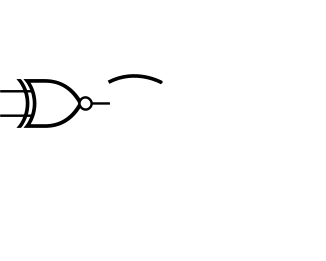
\includegraphics[scale=0.7]{figuras/map-xnor.png}
  \caption{Mapeo de funciones lógicas a celdas estándar}
  \label{fig:map-xnor}
\end{figure}

Es común elegir las celdas estándar según el tipo de aplicación a desarrollar. Existen celdas estandar que fueron diseñadas para bajo consumo, o alta velocidad, o de mínima área. También existe la posibilidad de diseñar celdas que busquen la mejor relación velocidad-consumo-area que puedan ser utilizadas en muchas aplicaciones. En circuitos integrados para sistemas alimentados a batería se intentará utilizar las celdas de menor consumo y evitar siempre que sea posible las de mayor velocidad, en función del presupuesto de potencia disponible para el mismo.

En nuestro caso, por la naturaleza del problema planteado, utilizamos una pequeña librería de celdas estándar diseñadas para tamaño mínimo de canal n, y p. %Una referencia al Rabaey es necesaria? 
Otra característica de la librería es la distancia entre el riel de VSS hasta el riel de VDD. Esta distancia es de 117 $\lambda$ (En nuestra tecnología de 180~$\mathrm{nm}$, el valor de lambda es: $\lambda = 100~\mathrm{nm}$), lo cual permite el ruteo horizontal de 16 pistas de metal por encima de las celdas, con metal 3 hasta capas superiories.

 

%http://cmosedu.com/cmos1/electric/electric.htm
% “Tiny-Chip” padframes [1.5 mm x 1.5 mm]

\section{Ubicación y Cableado (\emph{Place \& Route})}
Partimos desde la descripción estructural\footnote{El resultado de la síntesis hecha con lava es un netlist a nivel de compuerta, listo para ser usado por una herramienta de \emph{place \& route}Gate-level netlist vhdl.} del vhdl que producimos en el capítulo \ref{diseñoDigital}. De \emph{Electric} usaremos la herramienta llamada \emph{Silicon Compiler}, que se encarga de ubicar y conectar las celdas según el archivo vhdl. En el apéndice \ref{vhdlNetlist} mostramos el resultado de sintetizar a compuertas nuestro circuito. Las compuertas que se usan son compuertas lógicas genéricas, aún podemos modificar este netlist primero para hacer optimizaciones lógicas, que en nuestro caso esto no es conveniente ya que hemos elegido la arquitectura para lograr la mejor relación de compromiso entre velocidad y menor interconectividad. Otra optimización a realizar es eligiendo la fuerza de la celda.



\emph{place \& route}



Arquero para que este archivo pueda ser usado con Electric fué necesario hacer algunas modificaciones:
\begin{enumerate}
\item Reemplazar los nombres de las instancias de las celdas estándar que  seleccionamos en la sección \ref{celdasEstandars} y \emph{Electric} utilizará.
\item En la parte del vhdl que comienza la descripción estructural es necesario agregar las celdas estandar que serán utilizadas en el circuito.
\item Quitar todas las instancias de \verb|wire port map (...)| volviendo a conectar lo que queda desconectado al quitar estas instancias.
\end{enumerate}  
Estas tareas las realizamos modificando el código del programa de lava que crea el netlist vhdl llamado \verb|VhdlNew.hs|, y con un script\footnote{Adjuntamos el script en el apéndice \ref{scriptPerl}} en perl que es lanzado desde el mismo.
\subsection{Métricas de Calidad de un circuito digital}

Para cuantificar la calidad de un circuito, podemos analizar un circuito desde diferentes perspectivas: Costo, funcionalidad, robustez, performance y consumo de energía. Tomaremos estas dos últimas métricas, mas la del área (propiedad que define el costo) del circuito, para realizar la comparación entre las distintas arquitecturas analizadas.

\subsection{Performance}

\begin{figure}[h!]
\vspace{-5pt}
  \centering
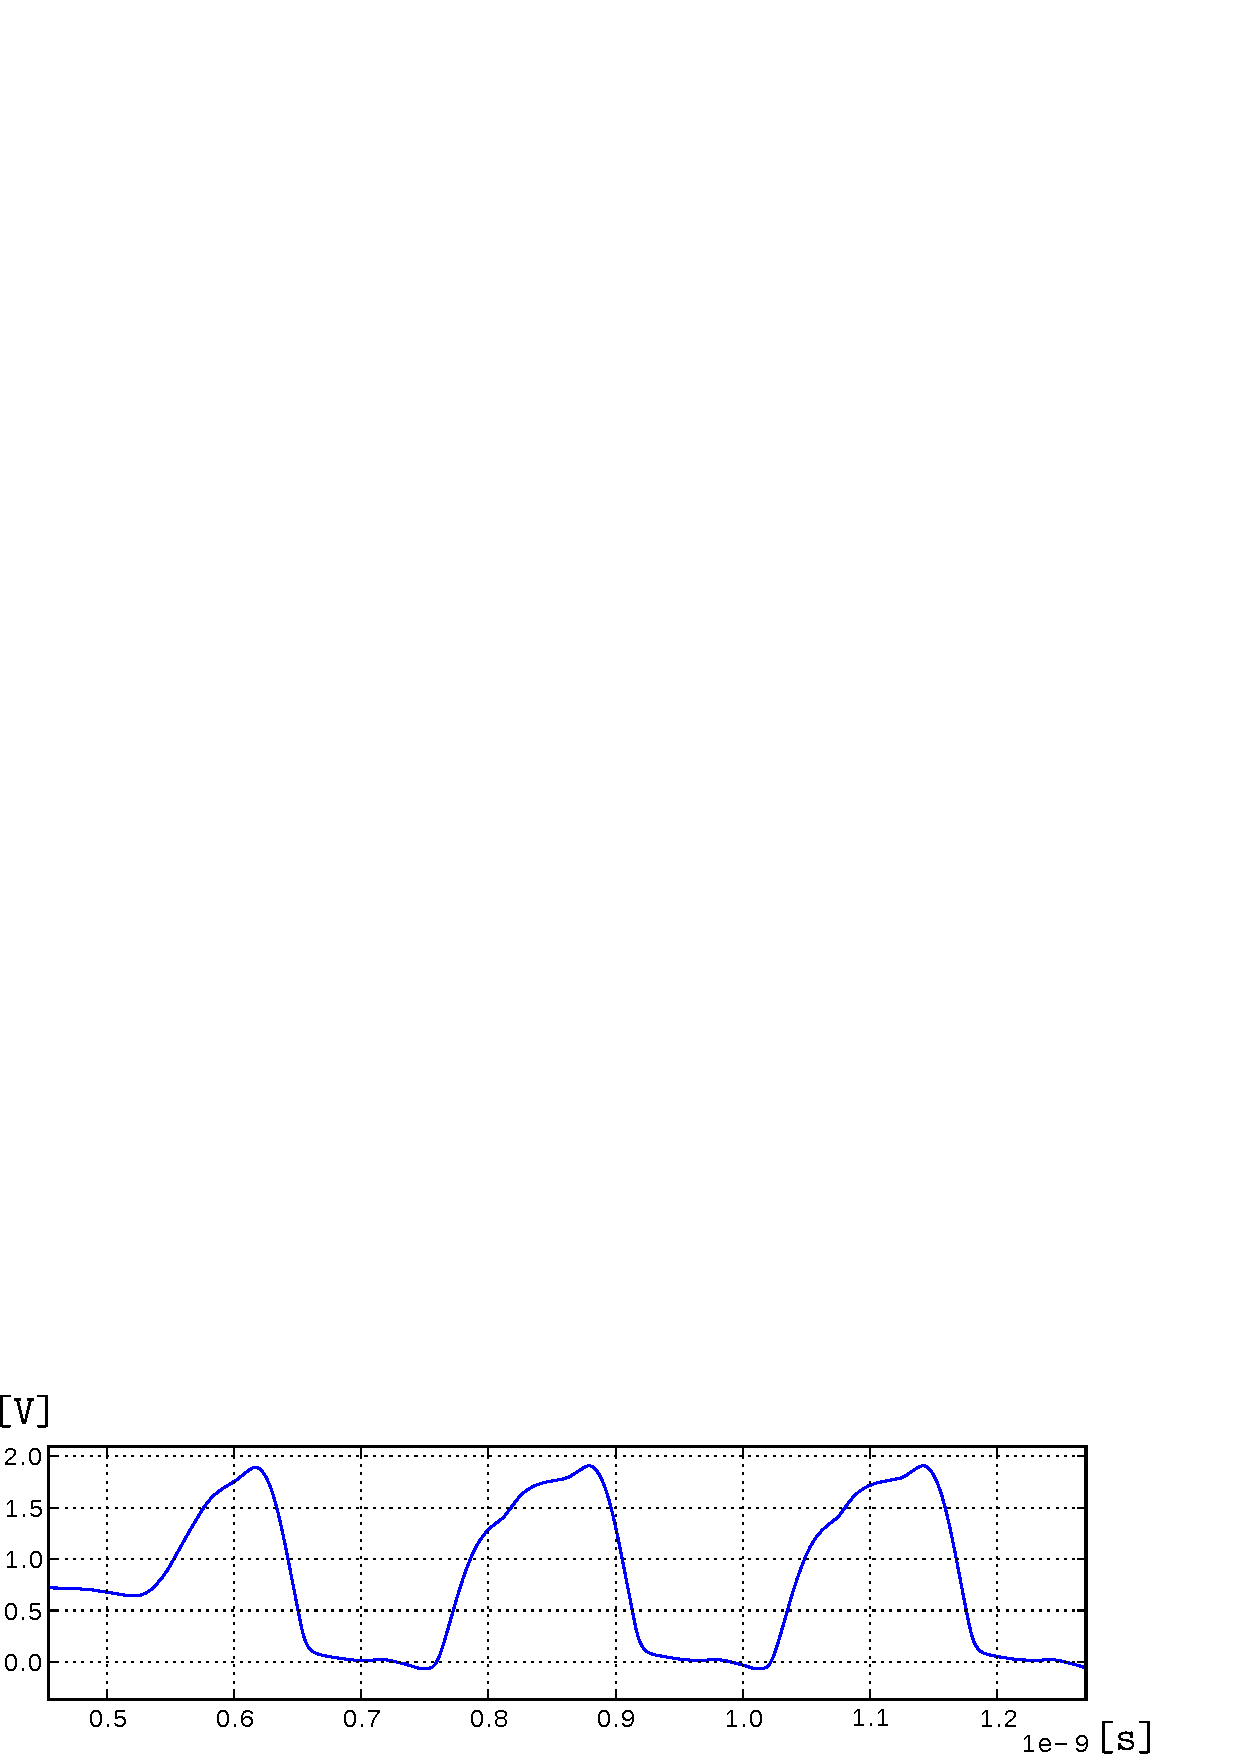
\includegraphics[scale=.3]{figuras/RO5.png}
  \caption{Layout del Oscilador anillo (N=5)}
\label{fig:RO5_lay}
\vspace{-10pt}
\end{figure}

Realizamos un oscilador anillo de 5 etapas, utilizando el inversor mas chico de nuestra librería de celdas estándar elegida. En la figura \ref{fig:RO5_lay} podemos ver el \emph{layout} que realizamos para esta prueba. Hacemos la extracción de parásitos y simulamos el circuito para obtener la forma de onda de la figura \ref{fig:RO5_wf}.

Como podemos deducir de la figura \ref{fig:RO5_wf}, el tiempo de propagación es de 32~pS, lo cual no significa que nuestros circuitos puedan correr a 31,25~GHz. Cuando medimos el tiempo de propagación usando este circuito, deberemos considerar que este es sólo una forma de comparar las tecnologías de fabricación y las topologías de las compuertas, pero de ninguna forma será la frecuencia máxima a la que pueda funcionar nuestro circuito, ya que la complejidad y cantidad de compuertas es enormemente mayor que la de un inversor. Según Rabaey\cite{rabaey2003} se puede esperar velocidades entre 50 a 100 veces mas bajas, aunque optimizando el diseño se puede lograr acercarnos un poco mas a esta frecuencia ideal. 

\begin{figure}[h!]
\vspace{-5pt}
  \centering
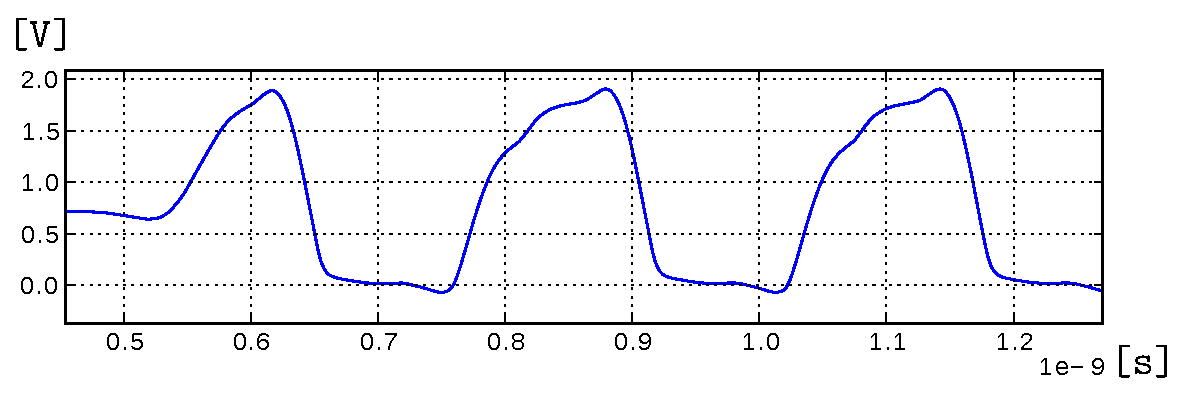
\includegraphics[scale=.6]{figuras/RO5.eps}
  \caption{Simulación con parásitos extraidos del layout de la figura \ref{fig:RO5_lay}}
\label{fig:RO5_wf}
\vspace{-10pt}
\end{figure}


\subsection{Tiempo mínimo de propagación}
t_p = 32 p

%Para simular corners: opConditions.lib


